

\section{Applications}

With Builder Marketplace’s omnichain infrastructure and intent-driven architecture, real-time multichain applications, once thought to be impossible, are now becoming a reality. This unlocks entirely new market segments and possibilities. Imagine Digital Forex markets with near-instant currency swaps at a fraction of traditional costs, or social application ecosystems where user data, identity, and assets flow seamlessly across platforms. Composable AI agents can now access and act on real-time data across protocols, enabling autonomous decision-making for tasks like trading, lending, or governance. Meanwhile, distributed settlement applications can coordinate complex, multi-party transactions across chains with trustless execution. These are just a few examples of the diverse and powerful applications that Builder Marketplace enables, ushering in a new era of connected, intelligent, and decentralized Web3 systems.

\subsection{Digital Forex}

Builder Marketplace introduces a powerful use case for digital currencies through Digital Forex, a low-cost, high-efficiency solution for global currency exchange using blockchain technology.

At the core of this innovation are Tether Tokens, which are digital assets that move seamlessly across blockchains while being pegged 1:1 to real-world currencies. These stablecoins offer price stability and reduced volatility, making them ideal for practical and everyday use in digital transactions. Tether currently supports several currencies, including: USDT (US Dollar), MXNT (Mexican Peso), CNHT (offshore Chinese Yuan), and XAUT (Gold).

\begin{figure}[h!]
    \centering
    \fbox{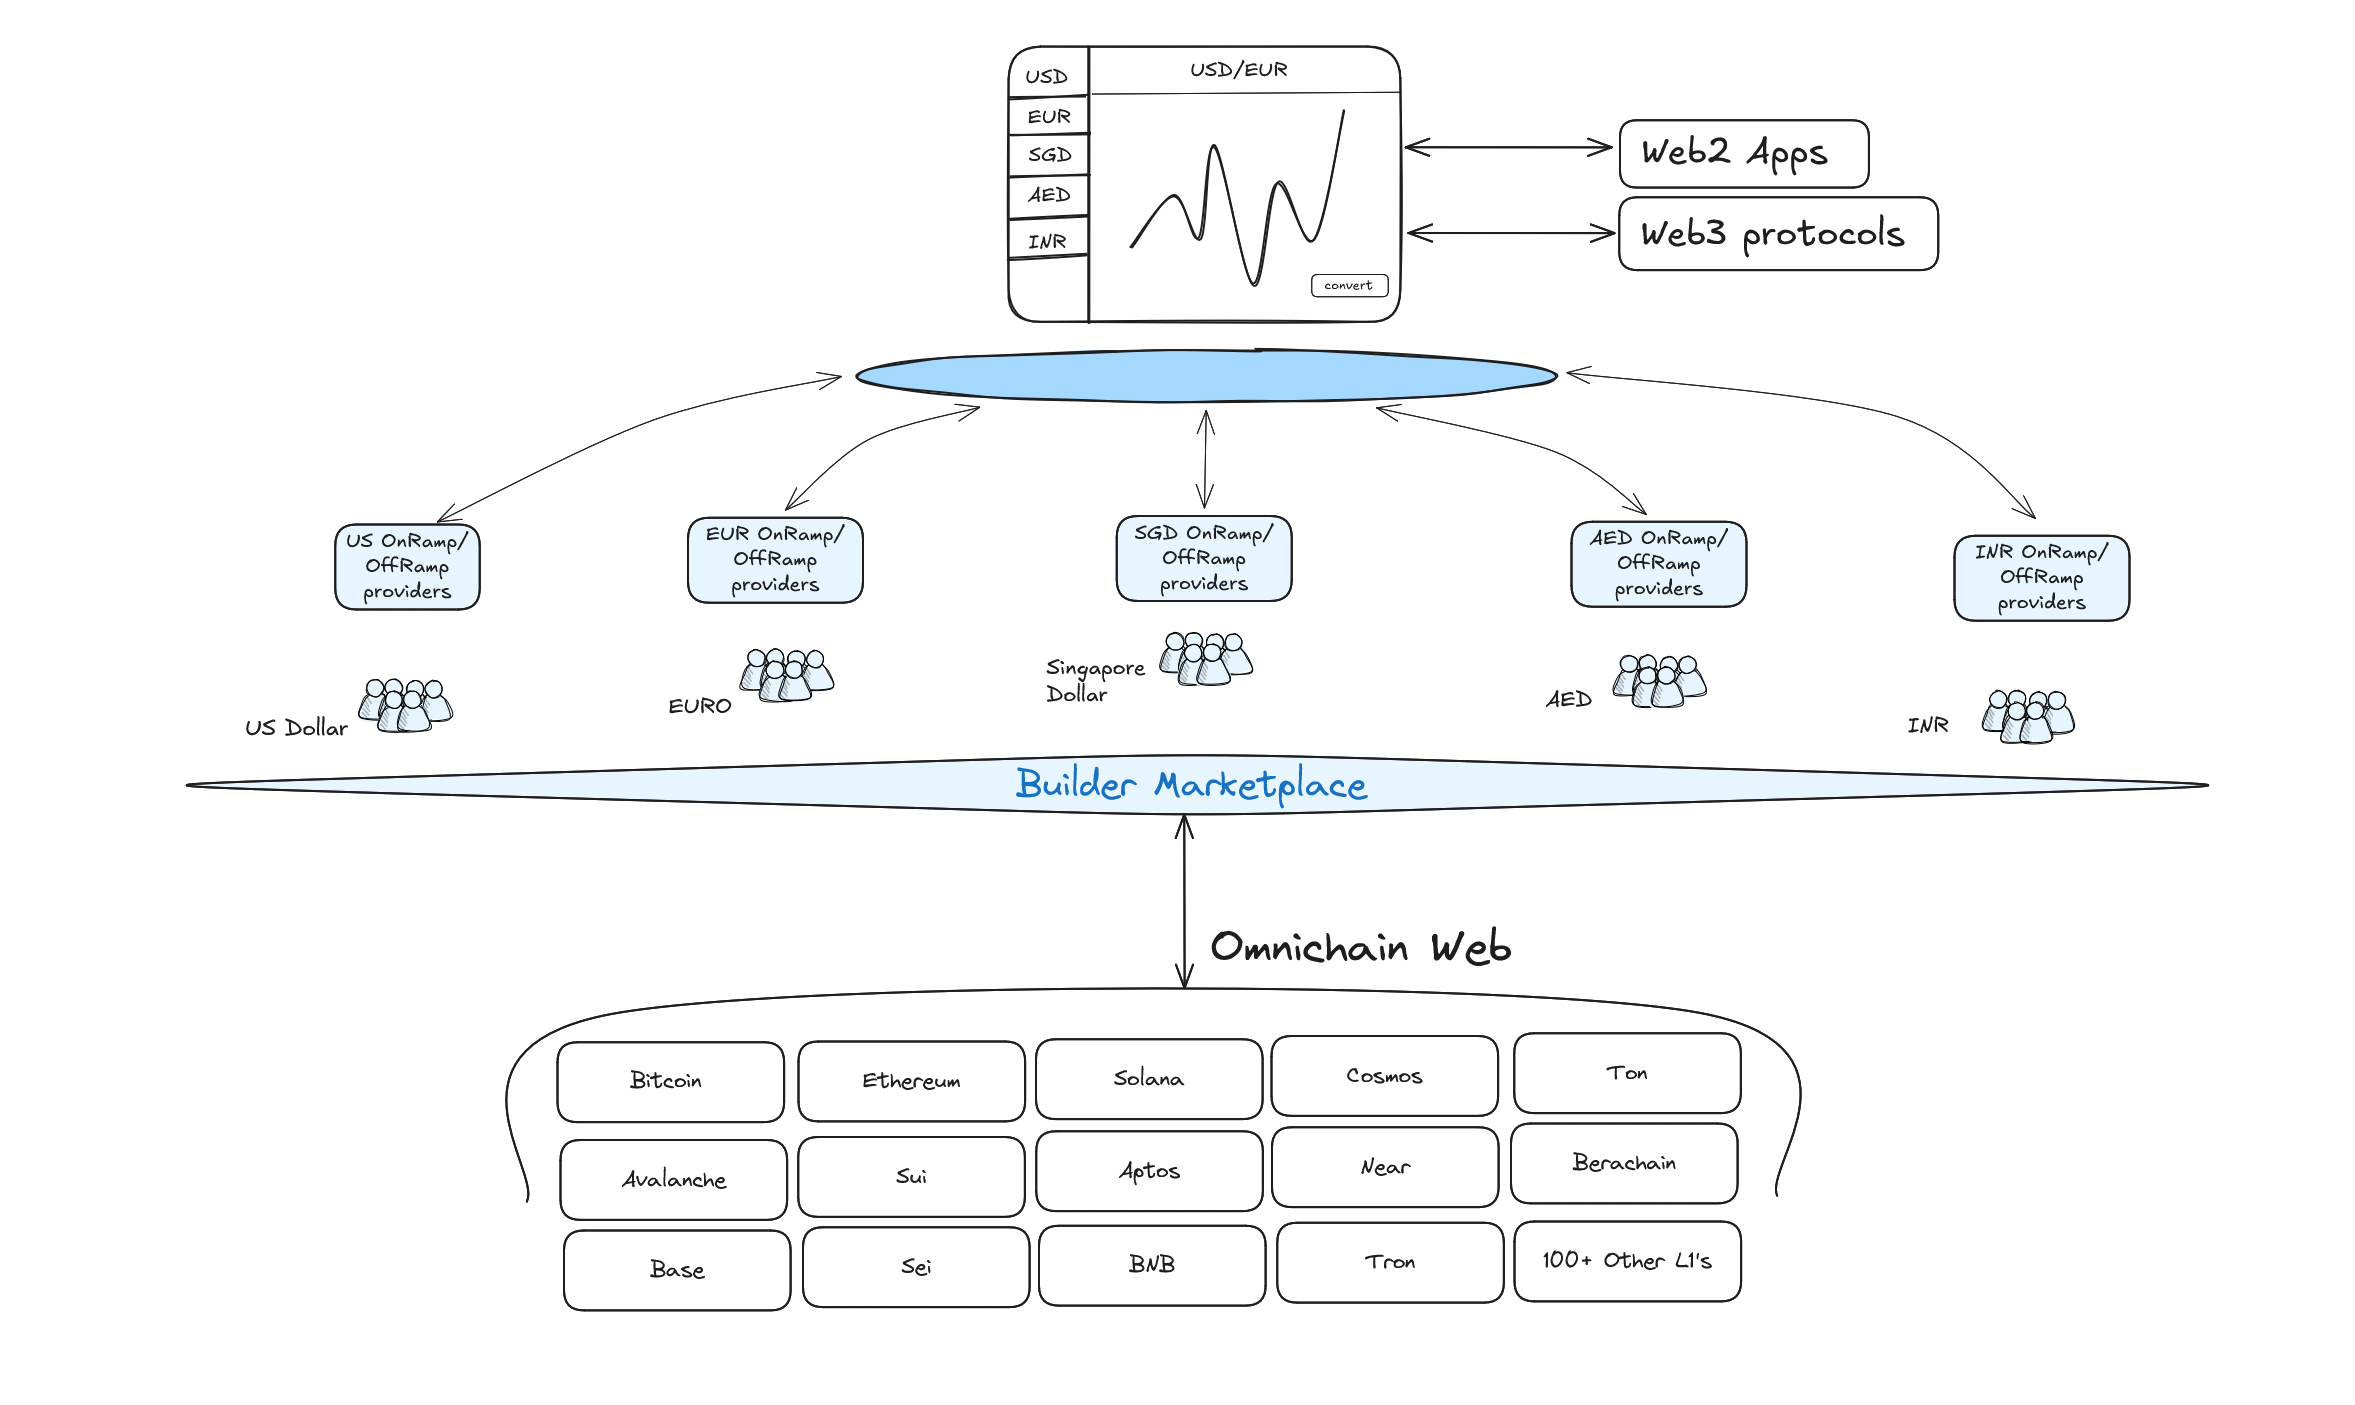
\includegraphics[width=0.99\linewidth]{figure/digital_forex.png}}
    \caption{Digital Forex Illustration}
    \label{fig:digitalforex}
\end{figure}

Traditional foreign exchange systems often impose transaction fees ranging from $1\%$ to $3\%$, making international currency exchanges expensive and inefficient. Digital Forex on Builder Marketplace addresses this by enabling currency exchange using stablecoins, reducing transaction fees to as low as $0.1\%$ in most cases.

\begin{itemize}
    \item[1.] On-Ramp/Off-Ramp Integration: Builder Marketplace integrates fiat on-ramp/off-ramp providers for each supported currency. These providers are connected to dedicated microchains that are capable of communicating with each other securely and efficiently.

    \item[2.] Seamless Cross-Currency Exchange: Users can deposit fiat currency (e.g., USD) through a USD on-ramp provider. This is converted into its digital equivalent (USDT) and transferred over the microchain network to the destination on-ramp/off-ramp provider for the target currency (e.g.CNHT). The user then receives the equivalent amount in fiat (Chinese Yuan) with minimal conversion costs.

    \item[3.] Web2 App Integration: A Web2 front-end can provide real-time exchange rates, allowing an intuitive interface for users to initiate and track currency conversions. The actual exchange of value is handled by the collaborating on-ramp/off-ramp providers, who settle the transaction in the digital currency layer using stablecoins.
\end{itemize}

By bringing together stablecoins, microchains and on-ramp / off-ramp providers, Builder Marketplace is creating a next-generation digital forex network, one that offers a secure, transparent, and cost-effective alternative to traditional foreign exchange systems.


\subsection{Intent Protocols and AI Agents}

As the Web3 ecosystem continues to expand, the demand for intent-driven architectures and solver networks is growing rapidly. However, without a shared infrastructure, these networks risk becoming isolated value silos, mirroring the same fragmentation that has long plagued traditional blockchains.

At Builder Marketplace, we address this challenge by offering a common interoperability layer that enables AI agents and intent protocols to operate seamlessly across chains, unifying access to data, protocols, and liquidity. AI agents are inherently intent-driven and data-dependent. They require continuous access to real-time information and actionable pathways across decentralized networks. However, the lack of standardization between fragmented blockchains restricts their ability to make informed decisions cross-chain.
\begin{figure}[h!]
    \centering
    \fbox{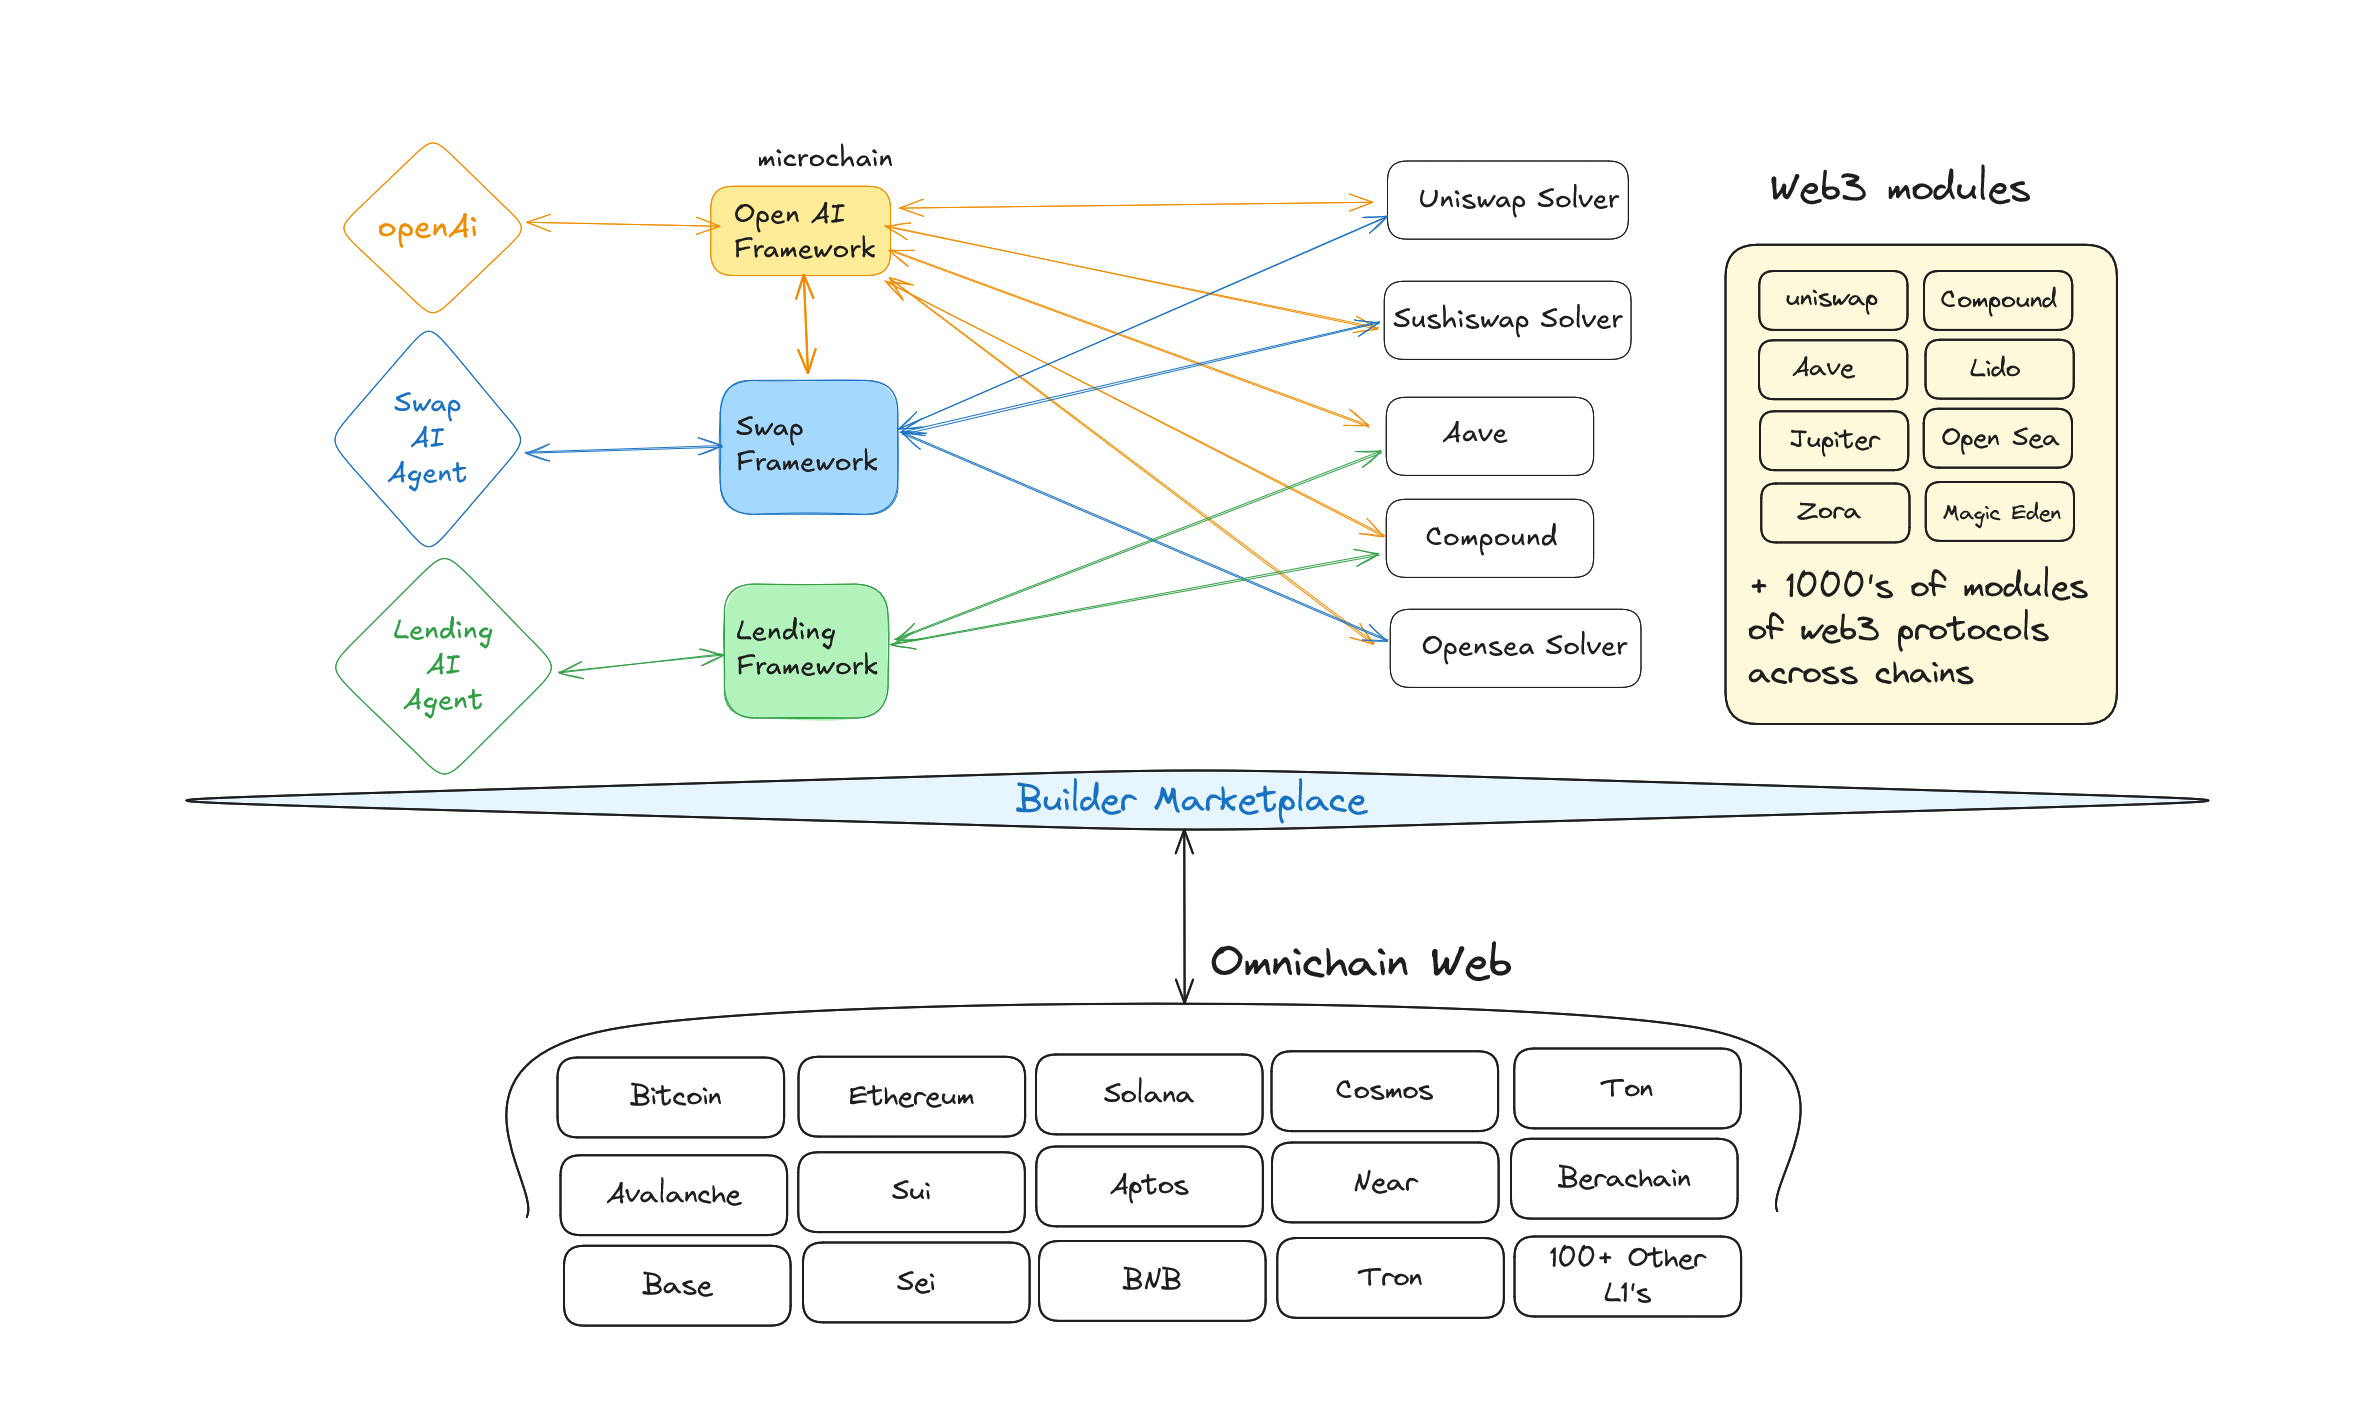
\includegraphics[width=0.99\linewidth]{figure/ai_agents.png}}
    \caption{AI Agents Illustration}
    \label{fig:aiagents}
\end{figure}
Builder Marketplace allows one to introduce a framework that defines a standard set of rules, data models, and logic for a particular type of AI agent or intent. For example:
\begin{itemize}
    \item Swap Framework: Gathers swap rates, gas prices, and slippage data from all integrated liquidity sources across chains. It builds a dynamic graph representation of the swap landscape, continuously updated to reflect the latest data. When a swap intent is received, the framework analyzes the graph to identify the most efficient route.

    \item Lending Framework: Evaluates interest rates and risk profiles across lending platforms like Compound, Aave, and Lido. Based on a user’s lending intent, it recommends the optimal strategy to maximize yield with minimum risk. 
\end{itemize}


These frameworks act as pluggable intelligence layers for AI agents, enabling them to understand the environment, evaluate multiple options, and act autonomously across the Web3 stack.

At the heart of this interoperability is Builder Marketplace’s support for modular Web3 integrations. We provide ready-to-use modules for major protocols such as: Uniswap, Aave, Compound, Lido, Jupiter and many more. Each module is designed to plug into relevant intent frameworks, enabling them to leverage the underlying cross-chain capabilities of the Omnichain Web, a universal data and execution layer that connects all microchains.

By offering an intent-native infrastructure with embedded cross-chain intelligence, Builder Marketplace becomes the launchpad for AI agents that can act on behalf of users, applications, and even DAOs—navigating the Web3 universe with autonomy and precision.
